% This template has been tested with LLNCS DOCUMENT CLASS -- version 2.20 (24-JUN-2015)

%"runningheads" enables:
%  - page number on page 2 onwards
%  - title/authors on even/odd pages
%This is good for other readers to enable proper archiving among other papers and pointing to
%content. Even if the title page states the title, when printed and stored in a folder, when
%blindly opening the folder, one could hit not the title page, but an arbitrary page. Therefore,
%it is good to have title printed on the pages, too.
\documentclass[runningheads,a4paper]{llncs}[2015/06/24]

%cmap has to be loaded before any font package (such as cfr-lm)
\usepackage{cmap}
\usepackage[T1]{fontenc}

\usepackage{graphicx}

% für neue deutsche Rechtschreibung
%\usepackage[english,ngerman]{babel}

% für englische Rechtschreibung
%Even though `american`, `english` and `USenglish` are synonyms for babel package (according to https://tex.stackexchange.com/questions/12775/babel-english-american-usenglish), the llncs document class is prepared to avoid the overriding of certain names (such as "Abstract." -> "Abstract" or "Fig." -> "Figure") when using `english`, but not when using the other 2.
%english has to go last to set it as default language
\usepackage[ngerman,english]{babel}

%Eingabeformat UTF-8
\usepackage[utf8]{inputenc}

%Hint by http://tex.stackexchange.com/a/321066/9075 -> enable "= as dashes
\addto\extrasenglish{\languageshorthands{ngerman}\useshorthands{"}}

%cfr-lm is preferred over lmodern. Reasoning at http://tex.stackexchange.com/a/247543/9075
\usepackage[%
rm={oldstyle=false,proportional=true},%
sf={oldstyle=false,proportional=true},%
tt={oldstyle=false,proportional=true,variable=true},%
qt=false%
]{cfr-lm}
%
%if more space is needed, exchange cfr-lm by mathptmx

\graphicspath{{graphics/}}

%Tweaks by IPVS/AS
\usepackage{lncs_as}

%for demonstration purposes only
\usepackage[math]{blindtext}

%Sorts the citations in the brackets
%It also allows \cite{refa, refb}. Otherwise, the document does not compile.
%  Error message: "White space in argument"
\usepackage{cite}


%% If you need packages for other papers,
%% START COPYING HERE
%% COPY ALSO cmap and fontenc from lines 10 to 12

%extended enumerate, such as \begin{compactenum}
\usepackage{paralist}

%put figures inside a text
%\usepackage{picins}
%use
%\piccaptioninside
%\piccaption{...}
%\parpic[r]{\includegraphics ...}
%Text...

%for easy quotations: \enquote{text}
\usepackage{csquotes}

%enable margin kerning
\usepackage{microtype}

%tweak \url{...}
\usepackage{url}
%\urlstyle{same}
%improve wrapping of URLs - hint by http://tex.stackexchange.com/a/10419/9075
\makeatletter
\g@addto@macro{\UrlBreaks}{\UrlOrds}
\makeatother
%nicer // - solution by http://tex.stackexchange.com/a/98470/9075
%DO NOT ACTIVATE -> prevents line breaks
%\makeatletter
%\def\Url@twoslashes{\mathchar`\/\@ifnextchar/{\kern-.2em}{}}
%\g@addto@macro\UrlSpecials{\do\/{\Url@twoslashes}}
%\makeatother

%diagonal lines in a table - http://tex.stackexchange.com/questions/17745/diagonal-lines-in-table-cell
%slashbox is not available in texlive (due to licensing) and also gives bad results. This, we use diagbox
%\usepackage{diagbox}

%required for pdfcomment later
\usepackage[hyperref,svgnames]{xcolor}

\usepackage{listings}
\lstloadlanguages{java}
\lstset{language=java,numbers=left,captionpos=b}


%enable nice comments
%this also loads hyperref
\usepackage{pdfcomment}
%enable hyperref without colors and without bookmarks
\hypersetup{hidelinks,
   colorlinks=true,
   allcolors=black,
   pdfstartview=Fit,
   breaklinks=true}
%enables correct jumping to figures when referencing
\usepackage[all]{hypcap}

\newcommand{\commentontext}[2]{\colorbox{yellow!60}{#1}\pdfcomment[color={0.234 0.867 0.211},hoffset=-6pt,voffset=10pt,opacity=0.5]{#2}}
\newcommand{\commentatside}[1]{\pdfcomment[color={0.045 0.278 0.643},icon=Note]{#1}}

%compatibality with packages todo, easy-todo, todonotes
\newcommand{\todo}[1]{\commentatside{#1}}
%compatiblity with package fixmetodonotes
\newcommand{\TODO}[1]{\commentatside{#1}}

%enable \cref{...} and \Cref{...} instead of \ref: Type of reference included in the link

%\usepackage[capitalise,nameinlink,ngerman]{cleveref}
\usepackage[capitalise,nameinlink,english]{cleveref}
%Nice formats for \cref - only for English texts
%\crefname{section}{Sect.}{Sect.}
%\Crefname{section}{Section}{Sections}

\usepackage{xspace}
%\newcommand{\eg}{e.\,g.\xspace}
%\newcommand{\ie}{i.\,e.\xspace}
\newcommand{\eg}{e.\,g.,\ }
\newcommand{\ie}{i.\,e.,\ }

%introduce \powerset - hint by http://matheplanet.com/matheplanet/nuke/html/viewtopic.php?topic=136492&post_id=997377
\DeclareFontFamily{U}{MnSymbolC}{}
\DeclareSymbolFont{MnSyC}{U}{MnSymbolC}{m}{n}
\DeclareFontShape{U}{MnSymbolC}{m}{n}{
    <-6>  MnSymbolC5
   <6-7>  MnSymbolC6
   <7-8>  MnSymbolC7
   <8-9>  MnSymbolC8
   <9-10> MnSymbolC9
  <10-12> MnSymbolC10
  <12->   MnSymbolC12%
}{}
\DeclareMathSymbol{\powerset}{\mathord}{MnSyC}{180}

% correct bad hyphenation here
\hyphenation{op-tical net-works semi-conduc-tor}

%% END COPYING HERE


\begin{document}

\title{Apache Storm}
%If Title is too long, use \titlerunning
%\titlerunning{Short Title}

\author{Aanal Raj Basaula}

\supervisor{Matthias Wieland}

\seminar{Advanced Topics in Data Management}

\semester{WS 2017/2018}

\abgabedatum{Stuttgart, 11.12.2017}

\institute{\email{aanal.basaula@gmail.com}}

%\frontpagede % creates the frontpage (in German)
\frontpageen % creates the frontpage (in English)

\thispagestyle{empty}
\cleardoublepage

\maketitle

\begin{abstract}
Apache Storm is one of the available open source tools for Stream Data Processing. This document provides a brief overview of the intricacies of the Architecture of Storm and tends to proceed further on the details of considerations required to design a Solution based on Storm. The design considerations relating to deployment of Storm System as a Lambda or a Lambda-less Architecture and the sketch of the various internal components of Storm i.e. Bolts, Spouts. We consider a practical implementation of Storm to try and express the theoretical design considerations in practice. Finally we list out the other available tools and compare them to Storm with regard to Performance, Resilience and various other parameters.
\end{abstract}

\begin{keywords}
Apache Storm, Stream Processing, Real Time Processing, Big Data
\end{keywords}

\section{Introduction}

\textbf{Data} today is generated by a lot of devices that are connected to the internet and the amount of data being generated at any instance is increasing rapidly. These devices could include a personal computer, a smart phone, or even an embedded device. Due to the rapid adoption of Internet of Things, data is being generated at an unprecedented rate. The sheer volume of data generated and the rate at which it is being generated can be termed as Big Data. The word \textbf{Big Data} made it's appearance in 1998 SGI slide deck made by John Mashey and now is of interest to a lot of financial as well as research institutions.\cite{miningstatus}

Data can be considered the oil of this present age, because with huge amounts of data one can determine hidden patterns. A lot of companies utilize pattern recognition on big data to open opportunities for revenue generation whereas research institutions use it to discover patterns simply not observable by the human mind(simply due to the volume of data). The question on how to classify any data as big data can be answered by using the 3Vs: Volume, Variety and Velocity \cite{usingapachestorm}. Any data with big volume or variety (such as text, video, images, etc.) or that gets generated rapidly can be considered as big data. In this paper regarding \textbf{Apache Storm} we consider the third V of big data to be the influencing factor.

\textbf{Data Stream} is a sequence of data flowing from a source to a destination, for example a sensor reporting the temperature to a server. The sensor measures the temperature periodically and updates it to the server. Another example could also be the purchase requests of products in a shopping site. In all of these scenarios, the data is continuously being generated. Traditionally analyzing these types of data requires storage of these data onto persistence and later batch processing it to discern patterns as well as other useful information. But, with the help of \textbf{Apache Storm} we are able to process these data as they are generated with minimum latency.

This benefit could be a major game changer for many companies as Stream processing of data allows Real Time Analysis. As an example, an online store could monitor its purchase requests for best performing and least performing articles and could offer discounts on the articles not performing good to increase their sales volume. This small change could increase the gross income of a company and will surely be advantageous.

\section{Apache Storm: Concepts}
\label{sec:concepts}
A stream is a continuous flow of data from one point to the other. Stream Processing System works on these data streams, the task of these processing scheme may range from simple transformations to something as complex as event processing. In this present digitized world, people tend to post most of their thoughts and voices about topics on the web. These may be in the form of a long text, generally a webpage called blogs, or as a short post on a social networking site. An example of a social networking site is Twitter. In twitter, people tend to post short views about various things and at any moment there are a number of people posting onto twitter.

A company which is interested in analyzing the current outlook of the organization can decide to analyze these posts on twitter. The posts created by twitter users could now then be considered as Data Stream for the company. As seen in \ref{fig:example} various users generate posts on twitter, which is stored on the twitter servers. These tweets are used by the company to analyze the sentiment of the users and the Reporting UI represents the results to the respective interested party.

\begin{figure}
  \begin{center}
    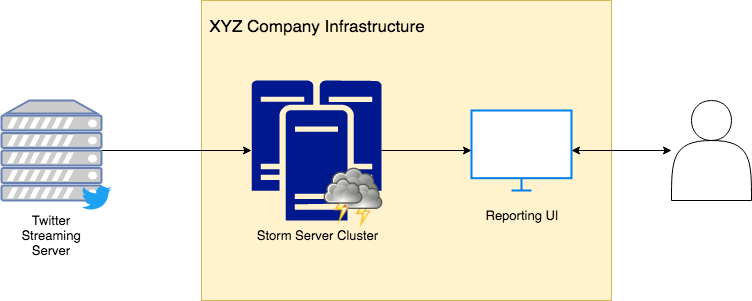
\includegraphics[width=\textwidth]{example.png}
    \caption{An Example Stream Processing Scenario}
    \label{fig:example}
   \end{center}
\end{figure}

Apache storm is one of the available open source tools for stream data processing, which is considered to be one of the simplest, fastest and fault tolerant systems available \cite{stormperspective}. These three factors have been the major points for the general public to choose \textbf{Apache Storm} above other available tools. It was originally created by Nathan Marz at BackType and till now, at present more than 60 companies \cite{stormtwitter} use or experiment with this tool.

\subsection{Architecture Overview}
The physical high level architecture of Storm as seen in figure \ref{fig:physicalarc} consists of a single master node and multiple worker nodes. The master node(see later) is the leader of the cluster and is responsible in short for the management of the different parts of the topology. There can only be one master node in a cluster. The worker node on the other hand is responsible for the actual execution of user logic. Storm requires at least one worker node to execute the user logic and apart from it a Zookeeper to keep track of the state of the various nodees in the cluster.

\begin{figure}
  \begin{center}
    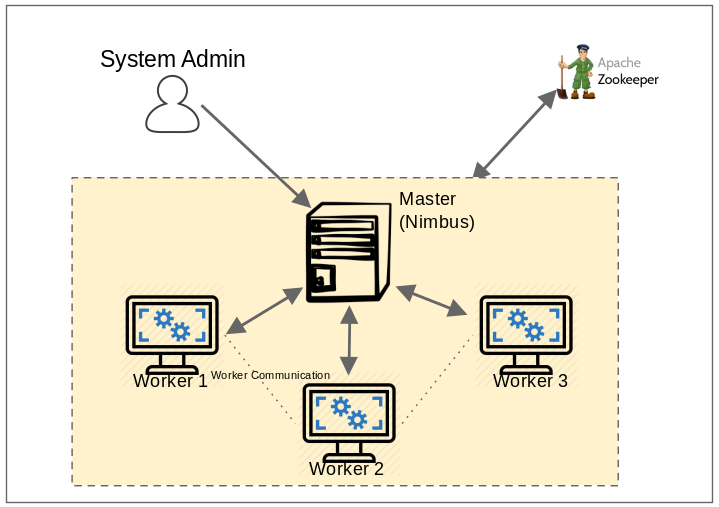
\includegraphics[width=.7\textwidth]{arch.png}
    \caption{Storm Physical Architecture}
    \label{fig:physicalarc}
   \end{center}
\end{figure}

The logical or the runtime architecture of storm is defined in storm via the abstraction of a topology. Topoloyg is a directed graph, with data flows and transformations to the flowing data. As seen in figure \ref{fig:topo} shows an example of a topology and consists of vertices and edges, the edges represent the flow of data whereas the vertices represent point where either data is generated or some processing to the existing data flowing throw it.

\subsubsection{Storm Components}
\paragraph{Master node} also called the \textbf{Nimbus} is responsible for the distribution and coordination of the execution of topologies. The Nimbus is the first point where the user submits the defined topology, which is then distributed among the worker nodes. The user submits the code as a jar file to the nimbus, nimbus then uses a combination of local disk and the zookeeper to store the topology defined in the jar file.\cite{stormtwitter} The topology thrift objects are stored in the zookeeper, whereas the code itself is stored in the local disk of nimbus. It then assigns the task to the worker nodes to execute selected parts of the topology.
\paragraph{Worker Node} is responsible for all the execution required for processing the incoming data stream. A worker node maintains a \textbf{Supervisor} process and multiple worker processes. The number of  worker processes depends upon the storm configurations and the number of woker nodes available. A worker process once spawned, starts working for a single topology alone and not for a multiple number of topologies. It creates threads called \textbf{Executors} which take up a tasks to be performed. A task for an executor is the vertex of the Directed graph. This can be observed in the \ref{fig:workerarch}, where a worker node has multiple worker processes, which in turn has multiple executors running different tasks. 
Even though storm can run multiple topologies, different processes may run separate topologies.

\paragraph{Supervisor} is part of a Worker Node and communicates with Nimbus and accepts incoming jobs. It monitors the health of the worker processes and respawns every process in case of failure. The supervisor performs three major periodic tasks, namely heartbeat, synchronize supervisor and sunchronize process.
The \textbf{heartbeat} event is scheduled every 15 seconds by the supervisor and in this event it reports to the nimbus that the worker node is alive and provides information about the available worker processes.\cite{stormtwitter} With this provided information, nimbus decides whether it can accept new jobs or not and depending upon the requirements, schedules jobs to be performed by the node. The \textbf{synchronize supervisor} event runs every 10 seconds and is reponsible for synchronization of the supervisor. It monitors the change is existing assignments and if the change includes an addition of topology, then downloads the required jar files and its dependencies and immediately schedules a synchronize worker process event.

The \textbf{synchronize worker process} event runs every 3 seconds and is responsible for managing worker processes. It reads worker heartbeats and classifies those workers with one of the labels, \textit{valid, timed out, not started or disallowed}.

\begin{figure}
  \begin{center}
    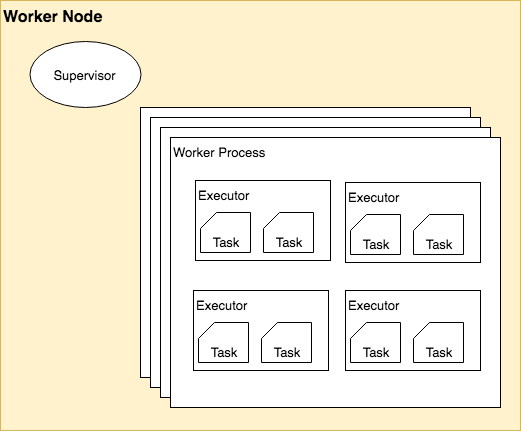
\includegraphics[width=.7\textwidth]{worker.png}
    \caption{Worker Node Architecture}
    \label{fig:workerarch}
   \end{center}
\end{figure}

\subsubsection{Topology}
\paragraph{Topology} is a directed graph where as mentioned before the vertices represent computation and the edges represent the data flow. It is wise to note that topologies in Storm are allowed to have cycles. The data in storm is abstracted using a Data type called the Tuple. A tuple is a list of ordered element, which as well contain names. The vertices of the topology can be abstracted into two different types, first the bolt and second the spout. \textbf{Spout} is the source of tuples into the topology whereas \textbf{Bolt} is a point in the topology where the tuples are transformed. A bolt typically does a simple transformation, in order to obtain a complex transformation, chaining of bolts can be done. 

The figure \ref{fig:topo} shows a basic Storm Topology with a single spout and three different bolts. The spout reads data from external sources, either homogenous or heterogenous and passes on to the bolts, according to the figure Bolt 1 and Bolt 2. Bolt 1 and Bolt 2 perform simple transformations and send the results to Bolt 3, which finalizes the data transformation and sends it to the Target. A topology as can be noted in the figure might have multiple instances of Bolts or Spouts running, which allows the scalability of the total system.

\begin{figure}
  \begin{center}
    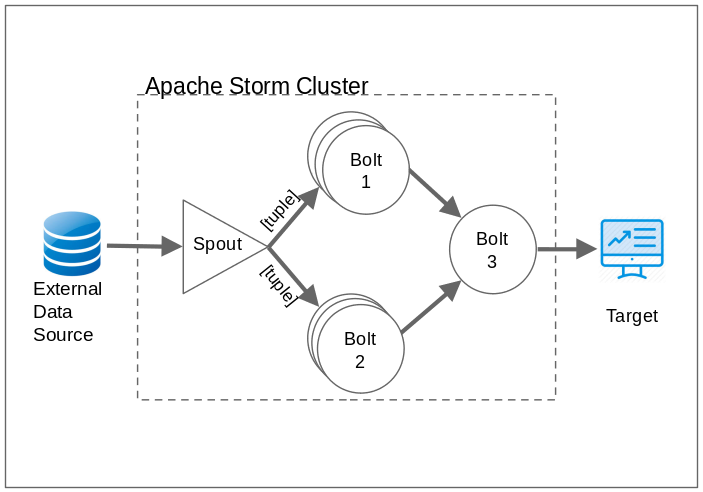
\includegraphics[width=0.85\textwidth]{topo.png}
    \caption{Generic Storm Topology}
    \label{fig:topo}
   \end{center}
\end{figure}

\paragraph{Multiple instances} of the same bolt is available within a topology, thus, Storm allows one to partition the data stream to the bolts, termed as Stream Grouping. There are eight available built-in stream groupings which can be used and custom extensions can be made according to the needs of the system.\footnote{\url{http://storm.apache.org/releases/1.1.0/Concepts.html}} The common built-in groupings are:

\begin{enumerate}
\item{Shuffle Grouping} : Random distribution of the tuples among the target nodes. Load balancing can be achieved using this grouping.
\item{Fields Grouping} : The tuples are partitioned by the value of a field. All the tuples with the same value of a specific field are routed to the same instance of the bolt. Can be used if a state of the bolt depends on the value of a field within the tuple.
\item{All Grouping} : The tuples are replicated to every instance of the bolt.
\item{Global Grouping} : The tuples are sent only to a single instance of the bolt.
\end{enumerate}

Each tuple is produced and consumed by bolts, but actual communication happens between the Worker processes. Each worker process has a Send thread and a Receive Thread which is responsible for handling the communication. As seen in figure \ref{fig:communication}, the Worker Receive thread receives messages from the global buffer and demultiplexes it to the respective tasks running in the User thread pool. Each User thread contains two message queues associated with it, the in-queue where incoming data is stored and the out-queue where the outgoing data is stored. The user thread, takes messages from the queue, processes them and sends them to the out queue. The data in the out queue is processed by the send queue and then passed on to the Worker Send Thread to be communicated into the network.

\begin{figure}
  \begin{center}
    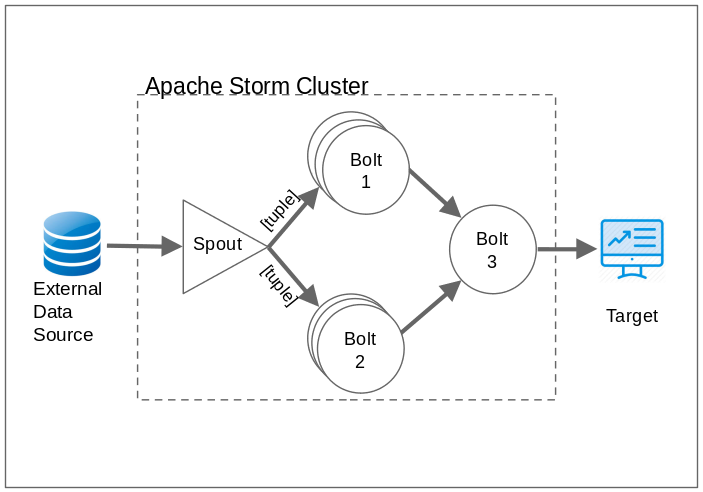
\includegraphics[width=\textwidth]{topo.png}
    \caption{Generic Storm Topology}
    \label{fig:communication}
   \end{center}
\end{figure}

\subsection{Storm Features}
Apache Storm has many features, some of them have been described in this section.
\subsubsection{Scalable}
\paragraph{Apache Storm} is a distributed system, and thus highly scalable. Adding of worker nodes in a storm is possible to increase the computational capacity of the total system. The concept of bolts with limited computations, allows one to increase the number of bolts performing a single task. For example, in a scenario where Bolt 1 parses text and Bolt 2 just counts occurrances, it is clear that Bolt 1 takes more time to process data rather than Bolt 2. So, increasing the number of Bolt 1 could be a better option in terms of scalability.

\subsubsection{Simple API}
\paragraph{Storm} provides a simple API for building on top of the pre-defined abstractions. Listing \ref{lst:spout} shows a bare bone implementation of a Spout. The Spout class extends the BaseRichSpout and implements only four methods, namely, declareOutputFields to declare the output fields this spout will be producing, open to handle initialization phase and close to handle the destroy phase and nextTuple to generate the next tuple. The API is similarly simple for implementing a Bolt. The complete detail of the API is out of the scope of this report and can be obtained from the official Storm documentation

\begin{lstlisting}[float,caption=Bare Spout Implementation,label=lst:spout]
public class TwitterFeedSpout extends BaseRichSpout {
	@Override
	public void declareOutputFields(OutputFieldsDeclarer declarer) {
	}
	
	@Override
	public void open(Map conf, TopologyContext context, 
	SpoutOutputCollector collector) {
	}

	@Override
	public void nextTuple() {
	}

	@Override
	public void close() {
	}
}
\end{lstlisting}

Another feature of the Storm API is that it supports multiple languages using JSON based protocol over Standard IO\footnote{\url{http://storm.apache.org/about/multi-language.html}}. This enables code reusability in most cases and makes it easier to port code into storm. 

\subsubsection{Fault Tolerance and Resilience}
\label{sec:resilience}
\paragraph{Apache storm} offers fault tolerance and resilience mechanisms with out of the box support and is tolerant against different types of failures. Nimbus, being the main master node, is in-charge of all the other worker nodes. Under the circumstance that a worker node fails, Nimbus re-spawns a worker node and assigns the tasks to this node. If the nimbus itself fails, the nimbus is not re-started automatically, but the worker nodes do not stop processing the stream. The nimbus can be later on restarted manually. During this phase, if a worker fails, it will not be restarted. The supervisor is also an active element within the Storm Architecture and keeps the Nimbus posted about it's current status. The \textbf{heartbeat} event is scheduled to run every 15 seconds and it reports to the Nimbus that the worker node is alive. \cite{stormtwitter}

\begin{figure}
  \begin{center}
    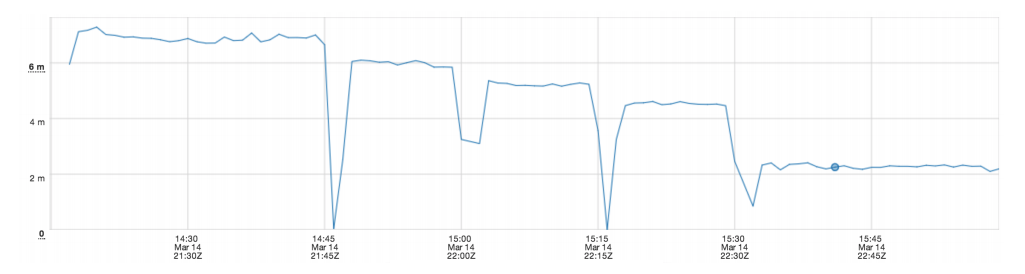
\includegraphics[width=\textwidth, height=0.25\textheight]{throughput.png}
    \caption{Throughput in time with respect to changing worker node availability \cite{stormtwitter}}
    \label{fig:throughput}
   \end{center}
\end{figure}

As we can see in figure \ref{fig:throughput}, an experiment conducted in \cite{stormtwitter} to check the resilience and performance of storm under loss of worker nodes. The worker nodes were turned off one by one in fixed durations, and the throughput of the system was measured at every instance. The durations and number of machines are shown below in table \ref{tab:experiment}. As seen, 3 machines were killed every 3 minutes, but the number of workers were limited to 50 at every instance, thus increasing the number of workers per machine. The graph \ref{fig:throughput} suggests that every 15 minutes, when the worker nodes were killed, the throughput was reduced significantly while storm tries to balance the topology again. The balancing does not require extensible amount of time and results into a new maximum throughput. As we can observe in the graph, the throughput decreases every time a node is removed, which is an expected phenomenon, due to the decrease in the computational capacity.

Apache Storm supports two types of processing schemes, \textbf{at least once} where each tuple is processed as the name suggests, and the other \textbf{at most once}, where the tuples are either processed once or dropped in cases of failure. To provide \textbf{at least once} semantics, Storm maintains an acker bolt, which keeps track of the tuple flow in the directed acyclic graph.

\begin{table}
\caption{Experimental setup during different time frames}
\label{tab:experiment}
\begin{center}
\begin{tabular}{r@{\quad}cl}
\hline
\multicolumn{1}{l}{\rule{0pt}{12pt} 
	Time}&\multicolumn{1}{l}{no of machines}\\[2pt]
\hline\rule{0pt}{12pt}
0 minutes  & 16  \\
+15 minutes & 13 \\
+30 minutes & 10 \\
+45 minutes & 7 \\
+60 mintues & 4 \\[2pt]
\hline
\end{tabular}
\end{center}
\end{table}

\begin{figure}
  \begin{center}
    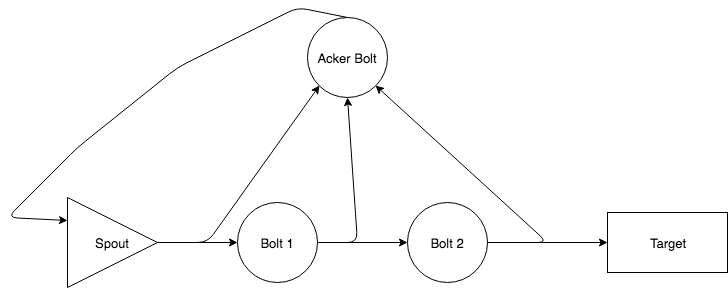
\includegraphics[width=.7\textwidth]{acker.png}
    \caption{Storm Acker Bolt \cite{stormtwitter}}
    \label{fig:acker}
   \end{center}
\end{figure}

\paragraph{Figure} \ref{fig:acker} shows the Acker bolt integration with the storm topology. It keeps track of the tuple flow starting from the point where it has been injected into the topology till it leaves the topology. After the tuple has left the topology, an \textbf{ack} is sent to the Spout, at this point, it removes the entry from memory.

\section{Practical Use Case}
\label{sec:usecase}
Apache Storm is used for stream processing of data, in many sources [2,3] a word frequency count example has been shown which can be considered to be trivial, but in actual practice it can be used to execute complicated algorithms. For the purposes of this paper we consider a trivial but different example of \textbf{Sentiment Analysis}.

\subsection{Scenario}

\subsubsection{Description}
\paragraph{Let us consider} a company which produces a range of products, for example \textbf{Apple Inc.} produces IPhones, IPods, MacBooks, etc. For such a big company an understanding of the sentiment of the people is important to maintain a positive outlook. The company can also analyze the feedback people place on a specific product, to change and adjust the pricing schemes in real time to the demand.  At present there are many social media networks available and people tend to share their views on these networks,  \textbf{Twitter}, for instance, is also one of these social networks where a number of posts are available publicly and can be analyzed to obtain a generalized view about a specific product or the company in general.

\subsubsection{Proposed Solution}

\paragraph{Solution} to the scenario can be implemented using \textbf{Apache Storm} to process the tweets in real time. Figure \ref{fig:example} shows the simplified system overview, consisting of Twitter Streaming Servers as the source of information. This information is processed in the Storm Clusters from within the Company Infrastructure and the analyzed result is reported to the User Interface, which can be accessed by the appropriate user.

\paragraph{This} is not the only possible solution, there are multiple other tools such as \textbf{Spark Streaming}, \textbf{Samza}, etc. but this paper concentrates Apache Storm as it is in the spotlight of this paper, for further details regarding other available tools and their comparisons with Apache Storm, please consider the section \ref{sec:toolcomparision} for further details.

\subsection{Practical Implementation}
The implementation of this solution concluded in three sub phases, namely Design, Development and Deployment. In the design phase, the storm topology was thoroughly planned, specifically the spouts, bolts and how they are interconnected. In the development phase, these spouts, bolts and other required aspects of the software were programmed and lastly deployed on a locally hosted storm server.

\subsubsection{Design}
\paragraph{Designing} a storm topology consists of determining the external sources of data (spouts), the processing that is required to this data imported from external sources (bolts) and the target system. Refer to figure \ref{fig:topoimpl} for the specific topology implementation for our use case. The sources of information for the scope of this paper is only Twitter Streaming API therefore a single Spout for integrating with the Twitter API is sufficient.

To Process the stream of tweets, we need to parse these tweets injected into the topology. The ParseTweetBolt processes these tweets and then emits whether the tweet was positive or negative under the simplified scenario. This separate positive or negative remark on a tweet does not provide useful information unless it is aggregated, thus a ResultAggregationBolt is responsible for aggregating all the results of the Parser bolt and providing the result to the target in real time.

\begin{figure}
  \begin{center}
    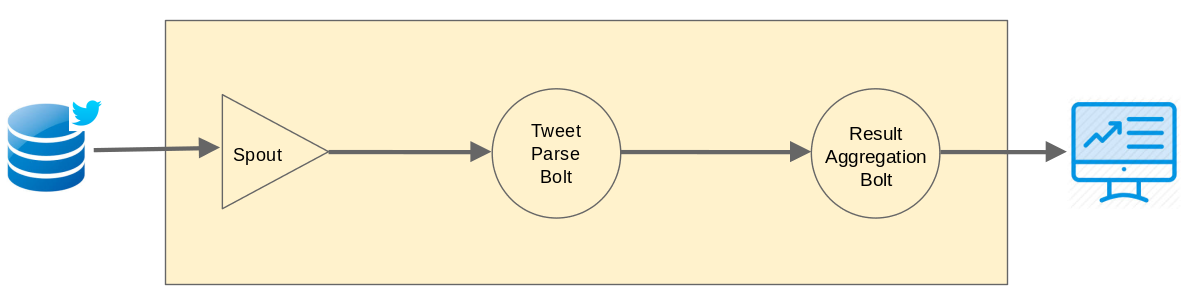
\includegraphics[width=.7\textwidth]{topoimpl.png}
    \caption{Topology Implementation for Sentiment Analysis}
    \label{fig:topoimpl}
   \end{center}
\end{figure}

The tweet spout contacts the twitter streaming server and fetches the available tweets in real time and relays it into the topology as a single tweet per tuple. The tuple is forwarded to the TweetParseBolt which will logically analyze the tweet as a positive or a negative tweet and with the percentage probability and emits this result to the ResultAggregationBolt. The ResultAggregationBolt calculates simply the weighted mean of the positive feedback and the negative feedbacks and outputs it into a local file, which can be later observed.

\subsubsection{Development}
\paragraph{Writing} code for storm can be achieved by using different programming languages depending upon the user. Apache Storm was designed to be usable with any programming languages\footnote{\url{http://storm.apache.org/about/multi-language.html}} and currently has Adapters available for Ruby, Python, Javascript and Perl.

The only spout available in this example uses Twitter Hosebird Client (\url{https://github.com/twitter/hbc}) to connect to Twitter Streaming Server and consume the Tweets generated in real time. Whereas the Bolts were programmed in java and the complete code can be viewed in \url{https://github.com/hakku276/storm-sentiment-analysis}. A short extract how the topology was created can be seen in listing  \ref{lst:toposetup}. We can see that a spout has been declared in line 2, then a parser bolt and finally a aggregator bolt with parallelism 1. It is then submitted to storm (nimbus).

\begin{lstlisting}[float,caption=Bare Spout Implementation,label=lst:toposetup]
TopologyBuilder builder = new TopologyBuilder();
builder.setSpout("spout", new TwitterFeedSpout(tags));
builder.setBolt("parse", new TweetParseBolt())
	.shuffleGrouping("spout");
builder.setBolt("aggregation", new TwitterAggregationBolt(), 1)
	.shuffleGrouping("parse");
StormSubmitter.submitTopology("SentimentAnalyzer", config, 
	builder.createTopology());
\end{lstlisting}

\subsection{Deployment}
\paragraph{Deploying} a storm topology requires a running zookeeper, nimbus and at least one worker node. In this practical implementation we use a single node to handle all the processing tasks. The zookeeper as well as the nimbus was instantiated in the local machine, along with a supervisor for the worker node. The Storm User interface presents all these information in a comprehensible manner within a web browser, which can be observed in figure \ref{fig:stormui}, the java code was compiled and packaged as a jar and submitted to nimbus for deployment (refer GitHub readme for further details). It was then deployed in storm, which can be observed in the Screen shot for the user interface in figure \ref{fig:stormui}.

\begin{figure}
  \begin{center}
    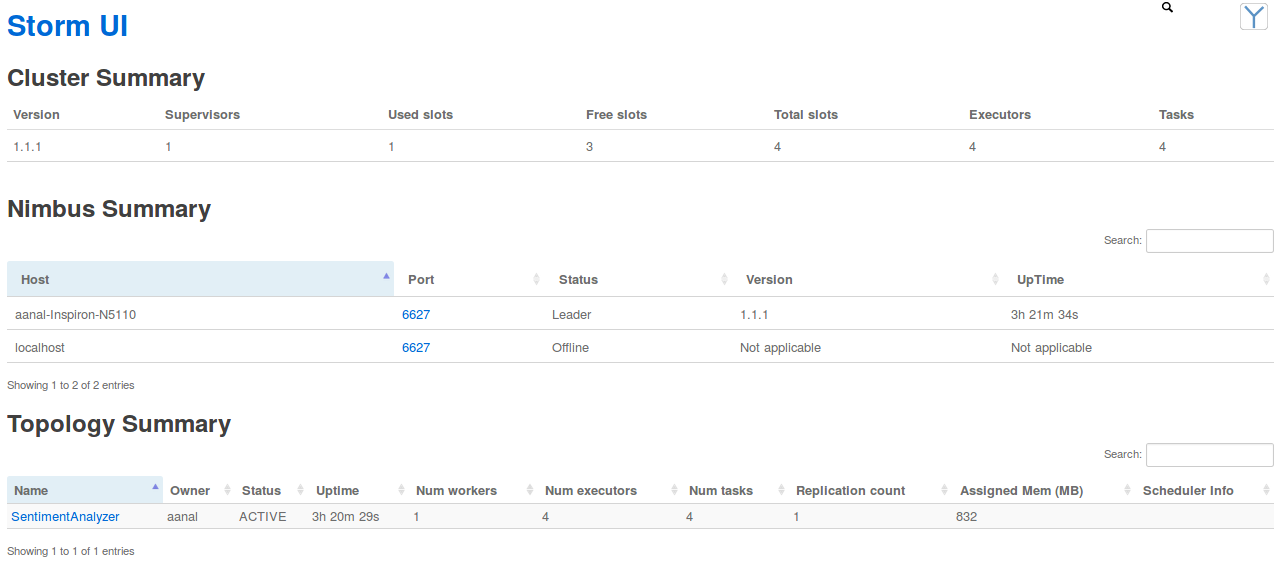
\includegraphics[width=\textwidth]{ui-mainpage.png}
    \caption{Main Page for Storm UI, displays all the cluster related details}
    \label{fig:stormui}
   \end{center}
\end{figure}

\section{Comparision to Related Work}
 \label{sec:toolcomparision}
Stream processing is a topic under constant focus at present and a lot of tools as well as models have been designed and created to support it. This section makes a comparison of the available widely accepted tools today.
 
 \begin{enumerate}
 \item \textbf{Spark Streaming} is an Open Source based project for stream processing.  It relies on cluster computing systems and operates on batches. The batch window in Spark Streaming is comparatively small thus allowing stream processing. It also provides flexibility to work in different programming languages such as Java, Scala and Python.
 \item \textbf{Apache Samza} is an Open Source project for near realtime distributed stream processing framework. It uses Apache Kafka for messaging and Apache Hadoop YARN for fault tolerance, processor isolation, security and resource management.\footnote{http://samza.apache.org/}
 \item \textbf{Flink Streaming} is also a Real time stream processing tool for distributed systems and builds batch processing on top of the Streaming engine.
 \end{enumerate}
 
 \subsubsection{Development and Testing}
All three tools provide their own API for development and testing. A comparision among these tools can be made on a basis of the programming languages supported, Apache Samza currently only supports JVM languages, whereas Spark Streaming supports Java, Scala and Python. Apache Storm on the other hand supports JVM as well as Non JVM languages which increases development speed, as the developers can choose their language according to their comfort. Apart from being able to choose a language for development, users can utilize existing code, thus allowing high portability.
 
 \subsubsection{Tool setup}
Setting up of the tool in Apache Storm requires minimum effort, achieved by downloading the zookeeper and storm binaries and unpacking them onto the computer. A minor configuration changes required attention, such as the location where zookeeper and storm would store data in. Apart from these details, it works perfectly out of the box. Along the same line, Spark Streaming follows a similar approach for tool setup and can be installed by simply downloading the tarball and unpacking it. Apache Samza on the other hand maintains a repository \url(https://github.com/apache/samza-hello-samza) which contains the scripts which installs and starts the requirement dependencies in the host.
 
 \subsubsection{Deployment}
Deployment of an artifact on Apache storm is relatively easy. For the java application, one compiles the sources with all the required dependencies into a jar file. The jar file can then be easily deployed into storm via a simple command.
 
 \subsubsection{Fault Tolerance}
As stream processing systems run for extended periods, it is quite necessary that these are able to handle various kinds of faults and still keep processing data as they enter the system. The fault tolerance model for Storm has been extensively described in section \ref{sec:resilience}. In cases of worker failure, as described earlier, Storm restarts the worker and if a tuple that is being processed by this node was lost, is again replayed. Similarly, Spark Streaming and Apache Samza also use various techniques to resolve issues while deployed. Spark Streaming uses parallel worker recovery which is possible with the help of RDDs and Apache Samza uses checkpointing to restore a failed state. Due to the parallel recovery of Spark Streaming, in my opinion it proves better in worker failure resilience, since Storm can recognize that a node has failed and can restart it, but it cannot know a tuple has been lost until the tuple has timed out. Time outs take extra time and results in slower processing.

In case of master node failure, Storm worker node continues to process incoming tuples, but in Spark, the worker nodes stop working when the master node fails until a new leader starts. This is an added bonus to Storm, since a failed master manual restart would reinstate the state of the system without changes. This is a better resilience feature than provided by Spark Streaming.

\begin{figure}
\begin{center}
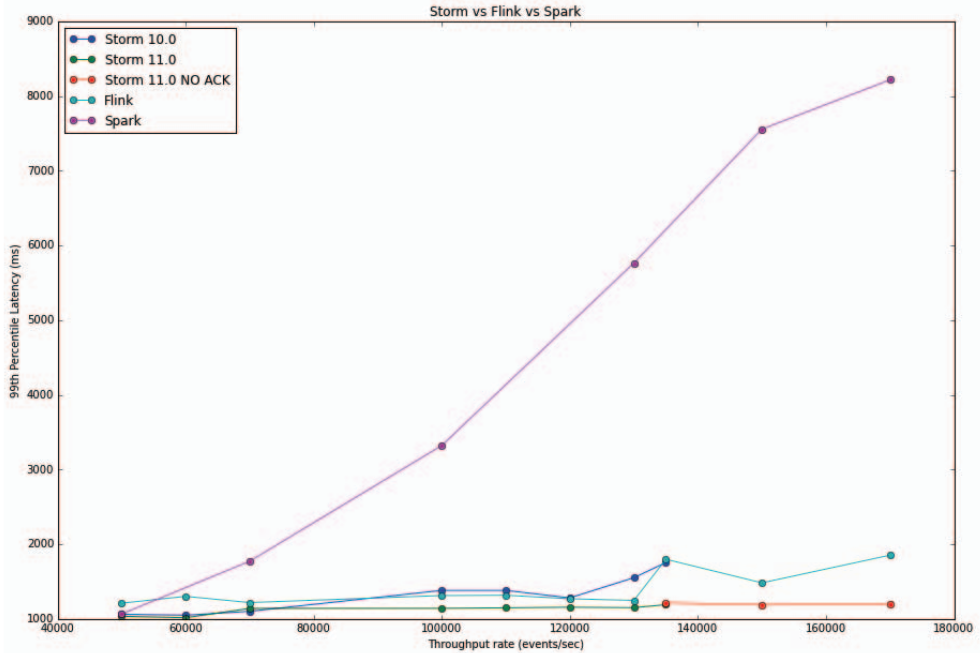
\includegraphics[width=0.85\textwidth]{comparisiongraph.png}
\caption{Performance Comparision between Apache Storm, Apache Flink and Spark Streaming \cite{benchmark}}
\label{fig:comparisiongraph}
\end{center}
\end{figure}
 
 \subsubsection{Benchmarks}
There has not been a comparative benchmark between Apache Storm, Spark Streaming and Apache Samza, but various sources have different comparisions between tools.  \cite{benchmark} considers Apache Storm, Spark Streaming and Apache Flink. The benchmark design consisted of counting the number of events taking place in the stream. The design was setup to read data from a Kafka Event Queue, the data being processed and result updated into Redis. The result included the window start time and the window end time, thus giving  an idea about the total latency of processing. According to this benchmark, they deduced that Apache Storm and Flink had low latency, whereas Spark Streaming had higher maximum throughput depending upon the batch duration setting. Figure \ref{fig:comparisiongraph} shows the comparative analysis among Apache Flink, Spark Streaming and Apache Storm. The batch processing scheme of Spark Streaming allows it to process events with higher throughput but with a trade off that the processing is delayed with higher latency. In the figure, we can observe that storm has comparatively less delay in processing, but according to \cite{benchmark}, storm with acking beyond 135,000 events per second, could not keep up with the throughput.
 
 \section{Discussion}
Apache Storm acts as a real time stream processing tool which is capable of computing results with high reliability and minimum latency. The tool is comparatively easy to setup and configure, with out of the box configurations which is production ready. The API is as well relatively simple and does not have a complicated method calls, the programming is based on event driven programming and since storm supports read and writes based on standard IO, utilizing previously written code could be relatively easier than in the other available tools. Data is currently being generated and consumed at an unprecedented rate, thus stream processing technologies is a requirement and is gaining popularity and attention. With all the various tools available, one can decide on which tool best suites ones needs. According to the benchmarks, if minimum latency is required, Apache Storm or Apache Flink or any system. Whereas if high throughput is required with a non strict latency criteria, Spark streaming could prove to be a better option.


%%%%%%%%%%%%%%%%%%%%%%%%%%%%%%%%%%%%%%%%%%%%%%%%%%%%%%%%%%%%%%%%%%%%%%%%%%%%%%%

\section{Bibliography}
\bibliographystyle{splncs03}
\bibliography{paper}
All Links were verified at 10.01.2018
\end{document}
